\documentclass[1p]{elsarticle_modified}
%\bibliographystyle{elsarticle-num}

%\usepackage[colorlinks]{hyperref}
%\usepackage{abbrmath_seonhwa} %\Abb, \Ascr, \Acal ,\Abf, \Afrak
\usepackage{amsfonts}
\usepackage{amssymb}
\usepackage{amsmath}
\usepackage{amsthm}
\usepackage{scalefnt}
\usepackage{amsbsy}
\usepackage{kotex}
\usepackage{caption}
\usepackage{subfig}
\usepackage{color}
\usepackage{graphicx}
\usepackage{xcolor} %% white, black, red, green, blue, cyan, magenta, yellow
\usepackage{float}
\usepackage{setspace}
\usepackage{hyperref}

\usepackage{tikz}
\usetikzlibrary{arrows}

\usepackage{multirow}
\usepackage{array} % fixed length table
\usepackage{hhline}

%%%%%%%%%%%%%%%%%%%%%
\makeatletter
\renewcommand*\env@matrix[1][\arraystretch]{%
	\edef\arraystretch{#1}%
	\hskip -\arraycolsep
	\let\@ifnextchar\new@ifnextchar
	\array{*\c@MaxMatrixCols c}}
\makeatother %https://tex.stackexchange.com/questions/14071/how-can-i-increase-the-line-spacing-in-a-matrix
%%%%%%%%%%%%%%%

\usepackage[normalem]{ulem}

\newcommand{\msout}[1]{\ifmmode\text{\sout{\ensuremath{#1}}}\else\sout{#1}\fi}
%SOURCE: \msout is \stkout macro in https://tex.stackexchange.com/questions/20609/strikeout-in-math-mode

\newcommand{\cancel}[1]{
	\ifmmode
	{\color{red}\msout{#1}}
	\else
	{\color{red}\sout{#1}}
	\fi
}

\newcommand{\add}[1]{
	{\color{blue}\uwave{#1}}
}

\newcommand{\replace}[2]{
	\ifmmode
	{\color{red}\msout{#1}}{\color{blue}\uwave{#2}}
	\else
	{\color{red}\sout{#1}}{\color{blue}\uwave{#2}}
	\fi
}

\newcommand{\Sol}{\mathcal{S}} %segment
\newcommand{\D}{D} %diagram
\newcommand{\A}{\mathcal{A}} %arc


%%%%%%%%%%%%%%%%%%%%%%%%%%%%%5 test

\def\sl{\operatorname{\textup{SL}}(2,\Cbb)}
\def\psl{\operatorname{\textup{PSL}}(2,\Cbb)}
\def\quan{\mkern 1mu \triangleright \mkern 1mu}

\theoremstyle{definition}
\newtheorem{thm}{Theorem}[section]
\newtheorem{prop}[thm]{Proposition}
\newtheorem{lem}[thm]{Lemma}
\newtheorem{ques}[thm]{Question}
\newtheorem{cor}[thm]{Corollary}
\newtheorem{defn}[thm]{Definition}
\newtheorem{exam}[thm]{Example}
\newtheorem{rmk}[thm]{Remark}
\newtheorem{alg}[thm]{Algorithm}

\newcommand{\I}{\sqrt{-1}}
\begin{document}

%\begin{frontmatter}
%
%\title{Boundary parabolic representations of knots up to 8 crossings}
%
%%% Group authors per affiliation:
%\author{Yunhi Cho} 
%\address{Department of Mathematics, University of Seoul, Seoul, Korea}
%\ead{yhcho@uos.ac.kr}
%
%
%\author{Seonhwa Kim} %\fnref{s_kim}}
%\address{Center for Geometry and Physics, Institute for Basic Science, Pohang, 37673, Korea}
%\ead{ryeona17@ibs.re.kr}
%
%\author{Hyuk Kim}
%\address{Department of Mathematical Sciences, Seoul National University, Seoul 08826, Korea}
%\ead{hyukkim@snu.ac.kr}
%
%\author{Seokbeom Yoon}
%\address{Department of Mathematical Sciences, Seoul National University, Seoul, 08826,  Korea}
%\ead{sbyoon15@snu.ac.kr}
%
%\begin{abstract}
%We find all boundary parabolic representation of knots up to 8 crossings.
%
%\end{abstract}
%\begin{keyword}
%    \MSC[2010] 57M25 
%\end{keyword}
%
%\end{frontmatter}

%\linenumbers
%\tableofcontents
%
\newcommand\colored[1]{\textcolor{white}{\rule[-0.35ex]{0.8em}{1.4ex}}\kern-0.8em\color{red} #1}%
%\newcommand\colored[1]{\textcolor{white}{ #1}\kern-2.17ex	\textcolor{white}{ #1}\kern-1.81ex	\textcolor{white}{ #1}\kern-2.15ex\color{red}#1	}

{\Large $\underline{12n_{0327}~(K12n_{0327})}$}

\setlength{\tabcolsep}{10pt}
\renewcommand{\arraystretch}{1.6}
\vspace{1cm}\begin{tabular}{m{100pt}>{\centering\arraybackslash}m{274pt}}
\multirow{5}{120pt}{
	\centering
	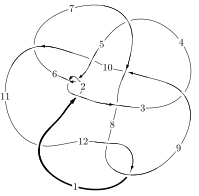
\includegraphics[width=112pt]{../../../GIT/diagram.site/Diagrams/png/2416_12n_0327.png}\\
\ \ \ A knot diagram\footnotemark}&
\allowdisplaybreaks
\textbf{Linearized knot diagam} \\
\cline{2-2}
 &
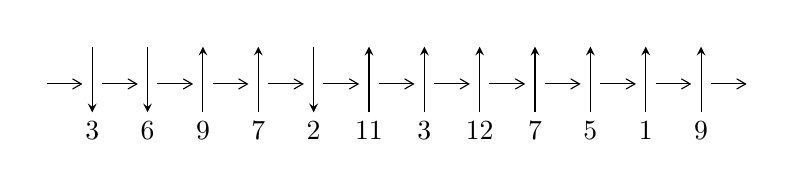
\begin{tikzpicture}[x=20pt, y=17pt]
	% nodes
	\node (C0) at (0, 0) {};
	\node (C1) at (1, 0) {};
	\node (C1U) at (1, +1) {};
	\node (C1D) at (1, -1) {3};

	\node (C2) at (2, 0) {};
	\node (C2U) at (2, +1) {};
	\node (C2D) at (2, -1) {6};

	\node (C3) at (3, 0) {};
	\node (C3U) at (3, +1) {};
	\node (C3D) at (3, -1) {9};

	\node (C4) at (4, 0) {};
	\node (C4U) at (4, +1) {};
	\node (C4D) at (4, -1) {7};

	\node (C5) at (5, 0) {};
	\node (C5U) at (5, +1) {};
	\node (C5D) at (5, -1) {2};

	\node (C6) at (6, 0) {};
	\node (C6U) at (6, +1) {};
	\node (C6D) at (6, -1) {11};

	\node (C7) at (7, 0) {};
	\node (C7U) at (7, +1) {};
	\node (C7D) at (7, -1) {3};

	\node (C8) at (8, 0) {};
	\node (C8U) at (8, +1) {};
	\node (C8D) at (8, -1) {12};

	\node (C9) at (9, 0) {};
	\node (C9U) at (9, +1) {};
	\node (C9D) at (9, -1) {7};

	\node (C10) at (10, 0) {};
	\node (C10U) at (10, +1) {};
	\node (C10D) at (10, -1) {5};

	\node (C11) at (11, 0) {};
	\node (C11U) at (11, +1) {};
	\node (C11D) at (11, -1) {1};

	\node (C12) at (12, 0) {};
	\node (C12U) at (12, +1) {};
	\node (C12D) at (12, -1) {9};
	\node (C13) at (13, 0) {};

	% arrows
	\draw[->,>={angle 60}]
	(C0) edge (C1) (C1) edge (C2) (C2) edge (C3) (C3) edge (C4) (C4) edge (C5) (C5) edge (C6) (C6) edge (C7) (C7) edge (C8) (C8) edge (C9) (C9) edge (C10) (C10) edge (C11) (C11) edge (C12) (C12) edge (C13) ;	\draw[->,>=stealth]
	(C1U) edge (C1D) (C2U) edge (C2D) (C3D) edge (C3U) (C4D) edge (C4U) (C5U) edge (C5D) (C6D) edge (C6U) (C7D) edge (C7U) (C8D) edge (C8U) (C9D) edge (C9U) (C10D) edge (C10U) (C11D) edge (C11U) (C12D) edge (C12U) ;
	\end{tikzpicture} \\
\hhline{~~} \\& 
\textbf{Solving Sequence} \\ \cline{2-2} 
 &
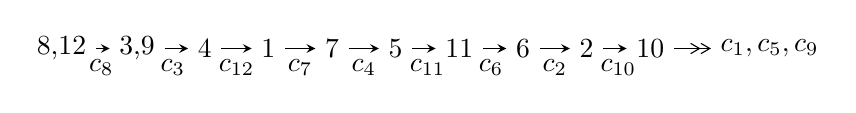
\begin{tikzpicture}[x=23pt, y=7pt]
	% node
	\node (A0) at (-1/8, 0) {8,12};
	\node (A1) at (17/16, 0) {3,9};
	\node (A2) at (17/8, 0) {4};
	\node (A3) at (25/8, 0) {1};
	\node (A4) at (33/8, 0) {7};
	\node (A5) at (41/8, 0) {5};
	\node (A6) at (49/8, 0) {11};
	\node (A7) at (57/8, 0) {6};
	\node (A8) at (65/8, 0) {2};
	\node (A9) at (73/8, 0) {10};
	\node (C1) at (1/2, -1) {$c_{8}$};
	\node (C2) at (13/8, -1) {$c_{3}$};
	\node (C3) at (21/8, -1) {$c_{12}$};
	\node (C4) at (29/8, -1) {$c_{7}$};
	\node (C5) at (37/8, -1) {$c_{4}$};
	\node (C6) at (45/8, -1) {$c_{11}$};
	\node (C7) at (53/8, -1) {$c_{6}$};
	\node (C8) at (61/8, -1) {$c_{2}$};
	\node (C9) at (69/8, -1) {$c_{10}$};
	\node (A10) at (11, 0) {$c_{1},c_{5},c_{9}$};

	% edge
	\draw[->,>=stealth]	
	(A0) edge (A1) (A1) edge (A2) (A2) edge (A3) (A3) edge (A4) (A4) edge (A5) (A5) edge (A6) (A6) edge (A7) (A7) edge (A8) (A8) edge (A9) ;
	\draw[->>,>={angle 60}]	
	(A9) edge (A10);
\end{tikzpicture} \\ 

\end{tabular} \\

\footnotetext{
The image of knot diagram is generated by the software ``\textbf{Draw programme}" developed by Andrew Bartholomew(\url{http://www.layer8.co.uk/maths/draw/index.htm\#Running-draw}), where we modified some parts for our purpose(\url{https://github.com/CATsTAILs/LinksPainter}).
}\phantom \\ \newline 
\centering \textbf{Ideals for irreducible components\footnotemark of $X_{\text{par}}$} 
 
\begin{align*}
I^u_{1}&=\langle 
7.90917\times10^{51} u^{45}+2.18534\times10^{51} u^{44}+\cdots+2.95768\times10^{53} b+5.20715\times10^{52},\\
\phantom{I^u_{1}}&\phantom{= \langle  }-7.60793\times10^{53} u^{45}-9.21427\times10^{53} u^{44}+\cdots+2.07037\times10^{54} a+1.08529\times10^{54},\;u^{46}+u^{45}+\cdots+20 u-7\rangle \\
I^u_{2}&=\langle 
- u^{15}+u^{14}+\cdots+b+1,\;-2 u^{15}-3 u^{14}+\cdots+a+4,\\
\phantom{I^u_{2}}&\phantom{= \langle  }u^{16}-5 u^{14}- u^{13}+13 u^{12}+3 u^{11}-23 u^{10}-6 u^9+29 u^8+8 u^7-26 u^6-8 u^5+16 u^4+4 u^3-6 u^2- u+1\rangle \\
\\
\end{align*}
\raggedright * 2 irreducible components of $\dim_{\mathbb{C}}=0$, with total 62 representations.\\
\footnotetext{All coefficients of polynomials are rational numbers. But the coefficients are sometimes approximated in decimal forms when there is not enough margin.}
\newpage
\renewcommand{\arraystretch}{1}
\centering \section*{I. $I^u_{1}= \langle 7.91\times10^{51} u^{45}+2.19\times10^{51} u^{44}+\cdots+2.96\times10^{53} b+5.21\times10^{52},\;-7.61\times10^{53} u^{45}-9.21\times10^{53} u^{44}+\cdots+2.07\times10^{54} a+1.09\times10^{54},\;u^{46}+u^{45}+\cdots+20 u-7 \rangle$}
\flushleft \textbf{(i) Arc colorings}\\
\begin{tabular}{m{7pt} m{180pt} m{7pt} m{180pt} }
\flushright $a_{8}=$&$\begin{pmatrix}1\\0\end{pmatrix}$ \\
\flushright $a_{12}=$&$\begin{pmatrix}0\\u\end{pmatrix}$ \\
\flushright $a_{3}=$&$\begin{pmatrix}0.367466 u^{45}+0.445053 u^{44}+\cdots-0.961201 u-0.524199\\-0.0267412 u^{45}-0.00738870 u^{44}+\cdots-0.488769 u-0.176055\end{pmatrix}$ \\
\flushright $a_{9}=$&$\begin{pmatrix}1\\- u^2\end{pmatrix}$ \\
\flushright $a_{4}=$&$\begin{pmatrix}0.365109 u^{45}+0.654340 u^{44}+\cdots-0.429450 u-0.157144\\0.164232 u^{45}-0.120965 u^{44}+\cdots+3.76063 u-1.65757\end{pmatrix}$ \\
\flushright $a_{1}=$&$\begin{pmatrix}u\\- u^3+u\end{pmatrix}$ \\
\flushright $a_{7}=$&$\begin{pmatrix}-0.236300 u^{45}+0.371650 u^{44}+\cdots-14.5049 u+8.55430\\0.359878 u^{45}+0.0463945 u^{44}+\cdots+4.16574 u-1.59970\end{pmatrix}$ \\
\flushright $a_{5}=$&$\begin{pmatrix}-0.296182 u^{45}+0.163568 u^{44}+\cdots+3.77995 u-0.792151\\0.358221 u^{45}-0.341011 u^{44}+\cdots+8.83971 u-4.10151\end{pmatrix}$ \\
\flushright $a_{11}=$&$\begin{pmatrix}- u^3\\u^5- u^3+u\end{pmatrix}$ \\
\flushright $a_{6}=$&$\begin{pmatrix}-0.0116433 u^{45}+0.300125 u^{44}+\cdots-9.16821 u+6.98444\\0.144819 u^{45}+0.138605 u^{44}+\cdots-1.99873 u+0.550517\end{pmatrix}$ \\
\flushright $a_{2}=$&$\begin{pmatrix}0.797806 u^{45}+0.285789 u^{44}+\cdots+9.18124 u+0.589049\\-0.315736 u^{45}+0.0205995 u^{44}+\cdots-5.78048 u+0.658747\end{pmatrix}$ \\
\flushright $a_{10}=$&$\begin{pmatrix}-0.185941 u^{45}-0.174269 u^{44}+\cdots+9.41906 u-2.70922\\-0.0739068 u^{45}-0.292990 u^{44}+\cdots+0.996475 u-1.61521\end{pmatrix}$\\&\end{tabular}
\flushleft \textbf{(ii) Obstruction class $= -1$}\\~\\
\flushleft \textbf{(iii) Cusp Shapes $= 1.28396 u^{45}+1.62893 u^{44}+\cdots-44.8335 u+13.8636$}\\~\\
\newpage\renewcommand{\arraystretch}{1}
\flushleft \textbf{(iv) u-Polynomials at the component}\newline \\
\begin{tabular}{m{50pt}|m{274pt}}
Crossings & \hspace{64pt}u-Polynomials at each crossing \\
\hline $$\begin{aligned}c_{1}\end{aligned}$$&$\begin{aligned}
&u^{46}+15 u^{45}+\cdots+2321 u+49
\end{aligned}$\\
\hline $$\begin{aligned}c_{2},c_{5}\end{aligned}$$&$\begin{aligned}
&u^{46}+3 u^{45}+\cdots-33 u+7
\end{aligned}$\\
\hline $$\begin{aligned}c_{3},c_{10}\end{aligned}$$&$\begin{aligned}
&u^{46}+u^{45}+\cdots+19 u+1
\end{aligned}$\\
\hline $$\begin{aligned}c_{4}\end{aligned}$$&$\begin{aligned}
&u^{46}+5 u^{45}+\cdots-2895 u-209
\end{aligned}$\\
\hline $$\begin{aligned}c_{6}\end{aligned}$$&$\begin{aligned}
&u^{46}-2 u^{45}+\cdots+15 u-19
\end{aligned}$\\
\hline $$\begin{aligned}c_{7}\end{aligned}$$&$\begin{aligned}
&u^{46}-3 u^{45}+\cdots-113405 u+77291
\end{aligned}$\\
\hline $$\begin{aligned}c_{8},c_{12}\end{aligned}$$&$\begin{aligned}
&u^{46}- u^{45}+\cdots-20 u-7
\end{aligned}$\\
\hline $$\begin{aligned}c_{9}\end{aligned}$$&$\begin{aligned}
&u^{46}+6 u^{45}+\cdots-75 u+9
\end{aligned}$\\
\hline $$\begin{aligned}c_{11}\end{aligned}$$&$\begin{aligned}
&u^{46}-33 u^{45}+\cdots-1366 u+49
\end{aligned}$\\
\hline
\end{tabular}\\~\\
\newpage\renewcommand{\arraystretch}{1}
\flushleft \textbf{(v) Riley Polynomials at the component}\newline \\
\begin{tabular}{m{50pt}|m{274pt}}
Crossings & \hspace{64pt}Riley Polynomials at each crossing \\
\hline $$\begin{aligned}c_{1}\end{aligned}$$&$\begin{aligned}
&y^{46}+53 y^{45}+\cdots-1065437 y+2401
\end{aligned}$\\
\hline $$\begin{aligned}c_{2},c_{5}\end{aligned}$$&$\begin{aligned}
&y^{46}-15 y^{45}+\cdots-2321 y+49
\end{aligned}$\\
\hline $$\begin{aligned}c_{3},c_{10}\end{aligned}$$&$\begin{aligned}
&y^{46}-63 y^{45}+\cdots-121 y+1
\end{aligned}$\\
\hline $$\begin{aligned}c_{4}\end{aligned}$$&$\begin{aligned}
&y^{46}-67 y^{45}+\cdots-133885 y+43681
\end{aligned}$\\
\hline $$\begin{aligned}c_{6}\end{aligned}$$&$\begin{aligned}
&y^{46}+2 y^{45}+\cdots-985 y+361
\end{aligned}$\\
\hline $$\begin{aligned}c_{7}\end{aligned}$$&$\begin{aligned}
&y^{46}-71 y^{45}+\cdots-125034513563 y+5973898681
\end{aligned}$\\
\hline $$\begin{aligned}c_{8},c_{12}\end{aligned}$$&$\begin{aligned}
&y^{46}-33 y^{45}+\cdots-1366 y+49
\end{aligned}$\\
\hline $$\begin{aligned}c_{9}\end{aligned}$$&$\begin{aligned}
&y^{46}-82 y^{45}+\cdots+5697 y+81
\end{aligned}$\\
\hline $$\begin{aligned}c_{11}\end{aligned}$$&$\begin{aligned}
&y^{46}-29 y^{45}+\cdots+39654 y+2401
\end{aligned}$\\
\hline
\end{tabular}\\~\\
\newpage\flushleft \textbf{(vi) Complex Volumes and Cusp Shapes}
$$\begin{array}{c|c|c}  
\text{Solutions to }I^u_{1}& \I (\text{vol} + \sqrt{-1}CS) & \text{Cusp shape}\\
 \hline 
\begin{aligned}
u &= -1.020210 + 0.218826 I \\
a &= \phantom{-}1.96292 + 1.78837 I \\
b &= -1.39819 - 1.19639 I\end{aligned}
 & \phantom{-}2.78540 - 4.43305 I & \phantom{-}7.31683 + 2.46379 I \\ \hline\begin{aligned}
u &= -1.020210 - 0.218826 I \\
a &= \phantom{-}1.96292 - 1.78837 I \\
b &= -1.39819 + 1.19639 I\end{aligned}
 & \phantom{-}2.78540 + 4.43305 I & \phantom{-}7.31683 - 2.46379 I \\ \hline\begin{aligned}
u &= \phantom{-}0.095870 + 1.057170 I \\
a &= \phantom{-}0.449277 - 0.228270 I \\
b &= \phantom{-}2.15949 - 0.25287 I\end{aligned}
 & \phantom{-}10.80880 + 1.13108 I & \phantom{-}8.33919 + 0.09433 I \\ \hline\begin{aligned}
u &= \phantom{-}0.095870 - 1.057170 I \\
a &= \phantom{-}0.449277 + 0.228270 I \\
b &= \phantom{-}2.15949 + 0.25287 I\end{aligned}
 & \phantom{-}10.80880 - 1.13108 I & \phantom{-}8.33919 - 0.09433 I \\ \hline\begin{aligned}
u &= -0.746943 + 0.560155 I \\
a &= \phantom{-}0.238979 - 0.456580 I \\
b &= -1.019220 + 0.072002 I\end{aligned}
 & \phantom{-}2.29880 + 1.44879 I & \phantom{-}7.06855 + 0.81086 I \\ \hline\begin{aligned}
u &= -0.746943 - 0.560155 I \\
a &= \phantom{-}0.238979 + 0.456580 I \\
b &= -1.019220 - 0.072002 I\end{aligned}
 & \phantom{-}2.29880 - 1.44879 I & \phantom{-}7.06855 - 0.81086 I \\ \hline\begin{aligned}
u &= \phantom{-}1.052910 + 0.350962 I \\
a &= \phantom{-}0.652736 + 0.849236 I \\
b &= \phantom{-}0.00161 - 1.51789 I\end{aligned}
 & \phantom{-}0.32230 + 4.17094 I & \phantom{-}4.61272 - 9.33404 I \\ \hline\begin{aligned}
u &= \phantom{-}1.052910 - 0.350962 I \\
a &= \phantom{-}0.652736 - 0.849236 I \\
b &= \phantom{-}0.00161 + 1.51789 I\end{aligned}
 & \phantom{-}0.32230 - 4.17094 I & \phantom{-}4.61272 + 9.33404 I \\ \hline\begin{aligned}
u &= -0.750943 + 0.440135 I \\
a &= \phantom{-}1.60823 + 1.02092 I \\
b &= -0.351616 + 1.000540 I\end{aligned}
 & -1.61798 - 2.21982 I & \phantom{-}4.07754 + 3.82774 I \\ \hline\begin{aligned}
u &= -0.750943 - 0.440135 I \\
a &= \phantom{-}1.60823 - 1.02092 I \\
b &= -0.351616 - 1.000540 I\end{aligned}
 & -1.61798 + 2.21982 I & \phantom{-}4.07754 - 3.82774 I\\
 \hline 
 \end{array}$$\newpage$$\begin{array}{c|c|c}  
\text{Solutions to }I^u_{1}& \I (\text{vol} + \sqrt{-1}CS) & \text{Cusp shape}\\
 \hline 
\begin{aligned}
u &= \phantom{-}1.17301\phantom{ +0.000000I} \\
a &= -2.66494\phantom{ +0.000000I} \\
b &= \phantom{-}1.80680\phantom{ +0.000000I}\end{aligned}
 & \phantom{-}9.52036\phantom{ +0.000000I} & \phantom{-}8.51710\phantom{ +0.000000I} \\ \hline\begin{aligned}
u &= -1.068340 + 0.517725 I \\
a &= \phantom{-}0.464086 + 1.138280 I \\
b &= -0.566866 - 0.471411 I\end{aligned}
 & \phantom{-}3.83816 - 4.69784 I & \phantom{-}11.69749 + 4.30932 I \\ \hline\begin{aligned}
u &= -1.068340 - 0.517725 I \\
a &= \phantom{-}0.464086 - 1.138280 I \\
b &= -0.566866 + 0.471411 I\end{aligned}
 & \phantom{-}3.83816 + 4.69784 I & \phantom{-}11.69749 - 4.30932 I \\ \hline\begin{aligned}
u &= \phantom{-}0.870642 + 0.823142 I \\
a &= -0.126114 + 0.358538 I \\
b &= \phantom{-}0.623928 + 0.125399 I\end{aligned}
 & -4.07204 + 3.05319 I & \phantom{-}15.3891 - 6.8553 I \\ \hline\begin{aligned}
u &= \phantom{-}0.870642 - 0.823142 I \\
a &= -0.126114 - 0.358538 I \\
b &= \phantom{-}0.623928 - 0.125399 I\end{aligned}
 & -4.07204 - 3.05319 I & \phantom{-}15.3891 + 6.8553 I \\ \hline\begin{aligned}
u &= -0.086683 + 1.203980 I \\
a &= -0.374986 + 0.103292 I \\
b &= -2.30710 - 0.06443 I\end{aligned}
 & \phantom{-}10.00560 + 7.40008 I & \phantom{-}7.39350 - 4.31642 I \\ \hline\begin{aligned}
u &= -0.086683 - 1.203980 I \\
a &= -0.374986 - 0.103292 I \\
b &= -2.30710 + 0.06443 I\end{aligned}
 & \phantom{-}10.00560 - 7.40008 I & \phantom{-}7.39350 + 4.31642 I \\ \hline\begin{aligned}
u &= -1.226800 + 0.055153 I \\
a &= -1.27654 - 0.97559 I \\
b &= \phantom{-}0.91044 + 1.53643 I\end{aligned}
 & \phantom{-}4.08578 + 2.48503 I & \phantom{-}10.70236 - 2.61783 I \\ \hline\begin{aligned}
u &= -1.226800 - 0.055153 I \\
a &= -1.27654 + 0.97559 I \\
b &= \phantom{-}0.91044 - 1.53643 I\end{aligned}
 & \phantom{-}4.08578 - 2.48503 I & \phantom{-}10.70236 + 2.61783 I \\ \hline\begin{aligned}
u &= -1.226440 + 0.133188 I \\
a &= -0.021931 - 0.272138 I \\
b &= -0.127594 - 0.708761 I\end{aligned}
 & \phantom{-}2.26273 - 2.31358 I & \phantom{-}11.62542 + 2.67684 I\\
 \hline 
 \end{array}$$\newpage$$\begin{array}{c|c|c}  
\text{Solutions to }I^u_{1}& \I (\text{vol} + \sqrt{-1}CS) & \text{Cusp shape}\\
 \hline 
\begin{aligned}
u &= -1.226440 - 0.133188 I \\
a &= -0.021931 + 0.272138 I \\
b &= -0.127594 + 0.708761 I\end{aligned}
 & \phantom{-}2.26273 + 2.31358 I & \phantom{-}11.62542 - 2.67684 I \\ \hline\begin{aligned}
u &= -1.106930 + 0.595666 I \\
a &= -0.835543 - 0.024113 I \\
b &= -0.293003 - 1.317840 I\end{aligned}
 & -0.37143 - 2.13318 I & \phantom{-}6.00000 + 0. I\phantom{ +0.000000I} \\ \hline\begin{aligned}
u &= -1.106930 - 0.595666 I \\
a &= -0.835543 + 0.024113 I \\
b &= -0.293003 + 1.317840 I\end{aligned}
 & -0.37143 + 2.13318 I & \phantom{-}6.00000 + 0. I\phantom{ +0.000000I} \\ \hline\begin{aligned}
u &= -0.283256 + 0.684205 I \\
a &= \phantom{-}0.210975 - 0.269709 I \\
b &= -0.682833 + 0.139746 I\end{aligned}
 & \phantom{-}1.63018 + 0.14156 I & \phantom{-}8.28809 + 0.51848 I \\ \hline\begin{aligned}
u &= -0.283256 - 0.684205 I \\
a &= \phantom{-}0.210975 + 0.269709 I \\
b &= -0.682833 - 0.139746 I\end{aligned}
 & \phantom{-}1.63018 - 0.14156 I & \phantom{-}8.28809 - 0.51848 I \\ \hline\begin{aligned}
u &= -0.019529 + 0.725158 I \\
a &= -0.777308 + 0.478111 I \\
b &= \phantom{-}0.500963 - 0.256778 I\end{aligned}
 & \phantom{-}0.47573 - 4.85542 I & \phantom{-}5.18911 + 6.50934 I \\ \hline\begin{aligned}
u &= -0.019529 - 0.725158 I \\
a &= -0.777308 - 0.478111 I \\
b &= \phantom{-}0.500963 + 0.256778 I\end{aligned}
 & \phantom{-}0.47573 + 4.85542 I & \phantom{-}5.18911 - 6.50934 I \\ \hline\begin{aligned}
u &= \phantom{-}1.260380 + 0.241271 I \\
a &= \phantom{-}1.265940 - 0.312252 I \\
b &= -1.138130 + 0.326314 I\end{aligned}
 & \phantom{-}6.24098 + 2.89108 I & \phantom{-0.000000 } 0 \\ \hline\begin{aligned}
u &= \phantom{-}1.260380 - 0.241271 I \\
a &= \phantom{-}1.265940 + 0.312252 I \\
b &= -1.138130 - 0.326314 I\end{aligned}
 & \phantom{-}6.24098 - 2.89108 I & \phantom{-0.000000 } 0 \\ \hline\begin{aligned}
u &= \phantom{-}0.640221 + 0.191594 I \\
a &= -1.51549 + 0.94495 I \\
b &= \phantom{-}0.776010 - 0.543436 I\end{aligned}
 & -1.81559 + 1.36574 I & \phantom{-}0.37681 - 4.32154 I\\
 \hline 
 \end{array}$$\newpage$$\begin{array}{c|c|c}  
\text{Solutions to }I^u_{1}& \I (\text{vol} + \sqrt{-1}CS) & \text{Cusp shape}\\
 \hline 
\begin{aligned}
u &= \phantom{-}0.640221 - 0.191594 I \\
a &= -1.51549 - 0.94495 I \\
b &= \phantom{-}0.776010 + 0.543436 I\end{aligned}
 & -1.81559 - 1.36574 I & \phantom{-}0.37681 + 4.32154 I \\ \hline\begin{aligned}
u &= \phantom{-}1.309540 + 0.386533 I \\
a &= -1.175660 + 0.376325 I \\
b &= \phantom{-}1.196350 - 0.295467 I\end{aligned}
 & \phantom{-}4.61382 + 9.03597 I & \phantom{-0.000000 } 0 \\ \hline\begin{aligned}
u &= \phantom{-}1.309540 - 0.386533 I \\
a &= -1.175660 - 0.376325 I \\
b &= \phantom{-}1.196350 + 0.295467 I\end{aligned}
 & \phantom{-}4.61382 - 9.03597 I & \phantom{-0.000000 } 0 \\ \hline\begin{aligned}
u &= \phantom{-}0.626188\phantom{ +0.000000I} \\
a &= \phantom{-}1.42934\phantom{ +0.000000I} \\
b &= \phantom{-}1.02581\phantom{ +0.000000I}\end{aligned}
 & \phantom{-}7.47324\phantom{ +0.000000I} & \phantom{-}21.6980\phantom{ +0.000000I} \\ \hline\begin{aligned}
u &= -1.37352 + 0.48037 I \\
a &= -1.81578 - 1.08493 I \\
b &= \phantom{-}2.71556 - 0.36369 I\end{aligned}
 & \phantom{-}15.4278 - 6.5327 I & \phantom{-0.000000 } 0 \\ \hline\begin{aligned}
u &= -1.37352 - 0.48037 I \\
a &= -1.81578 + 1.08493 I \\
b &= \phantom{-}2.71556 + 0.36369 I\end{aligned}
 & \phantom{-}15.4278 + 6.5327 I & \phantom{-0.000000 } 0 \\ \hline\begin{aligned}
u &= -0.538688\phantom{ +0.000000I} \\
a &= -0.314299\phantom{ +0.000000I} \\
b &= -0.326196\phantom{ +0.000000I}\end{aligned}
 & \phantom{-}0.769410\phantom{ +0.000000I} & \phantom{-}13.1770\phantom{ +0.000000I} \\ \hline\begin{aligned}
u &= \phantom{-}1.34301 + 0.58680 I \\
a &= -1.59637 + 1.02056 I \\
b &= \phantom{-}2.15155 + 1.01181 I\end{aligned}
 & \phantom{-}14.6331 + 4.7800 I & \phantom{-0.000000 } 0 \\ \hline\begin{aligned}
u &= \phantom{-}1.34301 - 0.58680 I \\
a &= -1.59637 - 1.02056 I \\
b &= \phantom{-}2.15155 - 1.01181 I\end{aligned}
 & \phantom{-}14.6331 - 4.7800 I & \phantom{-0.000000 } 0 \\ \hline\begin{aligned}
u &= -1.39068 + 0.61150 I \\
a &= \phantom{-}1.57695 + 1.08397 I \\
b &= -2.52625 + 0.71884 I\end{aligned}
 & \phantom{-}14.1038 - 13.8171 I & \phantom{-0.000000 } 0\\
 \hline 
 \end{array}$$\newpage$$\begin{array}{c|c|c}  
\text{Solutions to }I^u_{1}& \I (\text{vol} + \sqrt{-1}CS) & \text{Cusp shape}\\
 \hline 
\begin{aligned}
u &= -1.39068 - 0.61150 I \\
a &= \phantom{-}1.57695 - 1.08397 I \\
b &= -2.52625 - 0.71884 I\end{aligned}
 & \phantom{-}14.1038 + 13.8171 I & \phantom{-0.000000 } 0 \\ \hline\begin{aligned}
u &= \phantom{-}1.51006 + 0.50481 I \\
a &= \phantom{-}1.54874 - 0.74984 I \\
b &= -2.47250 - 0.79950 I\end{aligned}
 & \phantom{-}15.1375 - 1.1980 I & \phantom{-0.000000 } 0 \\ \hline\begin{aligned}
u &= \phantom{-}1.51006 - 0.50481 I \\
a &= \phantom{-}1.54874 + 0.74984 I \\
b &= -2.47250 + 0.79950 I\end{aligned}
 & \phantom{-}15.1375 + 1.1980 I & \phantom{-0.000000 } 0 \\ \hline\begin{aligned}
u &= \phantom{-}1.61183\phantom{ +0.000000I} \\
a &= \phantom{-}1.65979\phantom{ +0.000000I} \\
b &= -2.42384\phantom{ +0.000000I}\end{aligned}
 & \phantom{-}11.0760\phantom{ +0.000000I} & \phantom{-0.000000 } 0 \\ \hline\begin{aligned}
u &= \phantom{-}0.281467 + 0.135960 I \\
a &= -3.23232 - 0.74415 I \\
b &= \phantom{-}0.306108 + 0.706255 I\end{aligned}
 & -1.71245 - 1.30539 I & -1.21304 + 2.73809 I \\ \hline\begin{aligned}
u &= \phantom{-}0.281467 - 0.135960 I \\
a &= -3.23232 + 0.74415 I \\
b &= \phantom{-}0.306108 - 0.706255 I\end{aligned}
 & -1.71245 + 1.30539 I & -1.21304 - 2.73809 I\\
 \hline 
 \end{array}$$\newpage\newpage\renewcommand{\arraystretch}{1}
\centering \section*{II. $I^u_{2}= \langle - u^{15}+u^{14}+\cdots+b+1,\;-2 u^{15}-3 u^{14}+\cdots+a+4,\;u^{16}-5 u^{14}+\cdots- u+1 \rangle$}
\flushleft \textbf{(i) Arc colorings}\\
\begin{tabular}{m{7pt} m{180pt} m{7pt} m{180pt} }
\flushright $a_{8}=$&$\begin{pmatrix}1\\0\end{pmatrix}$ \\
\flushright $a_{12}=$&$\begin{pmatrix}0\\u\end{pmatrix}$ \\
\flushright $a_{3}=$&$\begin{pmatrix}2 u^{15}+3 u^{14}+\cdots-3 u-4\\u^{15}- u^{14}+\cdots-4 u-1\end{pmatrix}$ \\
\flushright $a_{9}=$&$\begin{pmatrix}1\\- u^2\end{pmatrix}$ \\
\flushright $a_{4}=$&$\begin{pmatrix}4 u^{15}+4 u^{14}+\cdots-6 u-8\\u^{15}- u^{14}+\cdots- u^2-3 u\end{pmatrix}$ \\
\flushright $a_{1}=$&$\begin{pmatrix}u\\- u^3+u\end{pmatrix}$ \\
\flushright $a_{7}=$&$\begin{pmatrix}2 u^{15}+u^{14}+\cdots+u+4\\-3 u^{15}-2 u^{14}+\cdots+2 u+3\end{pmatrix}$ \\
\flushright $a_{5}=$&$\begin{pmatrix}-5 u^{15}- u^{14}+\cdots+9 u+9\\u^{15}-4 u^{13}+\cdots+u+1\end{pmatrix}$ \\
\flushright $a_{11}=$&$\begin{pmatrix}- u^3\\u^5- u^3+u\end{pmatrix}$ \\
\flushright $a_{6}=$&$\begin{pmatrix}2 u^{15}+u^{14}+\cdots+u+4\\-3 u^{15}-2 u^{14}+\cdots+2 u+4\end{pmatrix}$ \\
\flushright $a_{2}=$&$\begin{pmatrix}3 u^{15}+6 u^{14}+\cdots+5 u-8\\-2 u^{15}-3 u^{14}+\cdots-3 u+3\end{pmatrix}$ \\
\flushright $a_{10}=$&$\begin{pmatrix}-2 u^{15}+11 u^{13}+\cdots-5 u-1\\6 u^{15}+3 u^{14}+\cdots-5 u-9\end{pmatrix}$\\&\end{tabular}
\flushleft \textbf{(ii) Obstruction class $= 1$}\\~\\
\flushleft \textbf{(iii) Cusp Shapes $= 4 u^{15}- u^{14}-21 u^{13}- u^{12}+59 u^{11}+11 u^{10}-107 u^9-31 u^8+137 u^7+47 u^6-125 u^5-54 u^4+74 u^3+30 u^2-23 u-3$}\\~\\
\newpage\renewcommand{\arraystretch}{1}
\flushleft \textbf{(iv) u-Polynomials at the component}\newline \\
\begin{tabular}{m{50pt}|m{274pt}}
Crossings & \hspace{64pt}u-Polynomials at each crossing \\
\hline $$\begin{aligned}c_{1}\end{aligned}$$&$\begin{aligned}
&u^{16}-8 u^{15}+\cdots-16 u+1
\end{aligned}$\\
\hline $$\begin{aligned}c_{2}\end{aligned}$$&$\begin{aligned}
&u^{16}+4 u^{15}+\cdots+4 u+1
\end{aligned}$\\
\hline $$\begin{aligned}c_{3}\end{aligned}$$&$\begin{aligned}
&u^{16}-10 u^{14}+\cdots-2 u-1
\end{aligned}$\\
\hline $$\begin{aligned}c_{4}\end{aligned}$$&$\begin{aligned}
&u^{16}+5 u^{13}+\cdots-8 u+1
\end{aligned}$\\
\hline $$\begin{aligned}c_{5}\end{aligned}$$&$\begin{aligned}
&u^{16}-4 u^{15}+\cdots-4 u+1
\end{aligned}$\\
\hline $$\begin{aligned}c_{6}\end{aligned}$$&$\begin{aligned}
&u^{16}- u^{15}+\cdots-4 u^2-1
\end{aligned}$\\
\hline $$\begin{aligned}c_{7}\end{aligned}$$&$\begin{aligned}
&u^{16}+4 u^{14}+\cdots-6 u+1
\end{aligned}$\\
\hline $$\begin{aligned}c_{8}\end{aligned}$$&$\begin{aligned}
&u^{16}-5 u^{14}+\cdots- u+1
\end{aligned}$\\
\hline $$\begin{aligned}c_{9}\end{aligned}$$&$\begin{aligned}
&u^{16}-7 u^{15}+\cdots+16 u-1
\end{aligned}$\\
\hline $$\begin{aligned}c_{10}\end{aligned}$$&$\begin{aligned}
&u^{16}-10 u^{14}+\cdots+2 u-1
\end{aligned}$\\
\hline $$\begin{aligned}c_{11}\end{aligned}$$&$\begin{aligned}
&u^{16}+10 u^{15}+\cdots+13 u+1
\end{aligned}$\\
\hline $$\begin{aligned}c_{12}\end{aligned}$$&$\begin{aligned}
&u^{16}-5 u^{14}+\cdots+u+1
\end{aligned}$\\
\hline
\end{tabular}\\~\\
\newpage\renewcommand{\arraystretch}{1}
\flushleft \textbf{(v) Riley Polynomials at the component}\newline \\
\begin{tabular}{m{50pt}|m{274pt}}
Crossings & \hspace{64pt}Riley Polynomials at each crossing \\
\hline $$\begin{aligned}c_{1}\end{aligned}$$&$\begin{aligned}
&y^{16}+20 y^{15}+\cdots-52 y+1
\end{aligned}$\\
\hline $$\begin{aligned}c_{2},c_{5}\end{aligned}$$&$\begin{aligned}
&y^{16}-8 y^{15}+\cdots-16 y+1
\end{aligned}$\\
\hline $$\begin{aligned}c_{3},c_{10}\end{aligned}$$&$\begin{aligned}
&y^{16}-20 y^{15}+\cdots+4 y+1
\end{aligned}$\\
\hline $$\begin{aligned}c_{4}\end{aligned}$$&$\begin{aligned}
&y^{16}-12 y^{14}+\cdots-20 y+1
\end{aligned}$\\
\hline $$\begin{aligned}c_{6}\end{aligned}$$&$\begin{aligned}
&y^{16}+9 y^{15}+\cdots+8 y+1
\end{aligned}$\\
\hline $$\begin{aligned}c_{7}\end{aligned}$$&$\begin{aligned}
&y^{16}+8 y^{15}+\cdots-10 y+1
\end{aligned}$\\
\hline $$\begin{aligned}c_{8},c_{12}\end{aligned}$$&$\begin{aligned}
&y^{16}-10 y^{15}+\cdots-13 y+1
\end{aligned}$\\
\hline $$\begin{aligned}c_{9}\end{aligned}$$&$\begin{aligned}
&y^{16}+9 y^{15}+\cdots-26 y+1
\end{aligned}$\\
\hline $$\begin{aligned}c_{11}\end{aligned}$$&$\begin{aligned}
&y^{16}+2 y^{15}+\cdots-17 y+1
\end{aligned}$\\
\hline
\end{tabular}\\~\\
\newpage\flushleft \textbf{(vi) Complex Volumes and Cusp Shapes}
$$\begin{array}{c|c|c}  
\text{Solutions to }I^u_{2}& \I (\text{vol} + \sqrt{-1}CS) & \text{Cusp shape}\\
 \hline 
\begin{aligned}
u &= -0.772761 + 0.712653 I \\
a &= \phantom{-}1.12093 + 0.97459 I \\
b &= \phantom{-}0.174212 + 0.983327 I\end{aligned}
 & -0.10256 - 4.89171 I & \phantom{-}5.59970 + 5.98315 I \\ \hline\begin{aligned}
u &= -0.772761 - 0.712653 I \\
a &= \phantom{-}1.12093 - 0.97459 I \\
b &= \phantom{-}0.174212 - 0.983327 I\end{aligned}
 & -0.10256 + 4.89171 I & \phantom{-}5.59970 - 5.98315 I \\ \hline\begin{aligned}
u &= \phantom{-}1.026470 + 0.385848 I \\
a &= -0.41213 + 1.88514 I \\
b &= \phantom{-}0.64749 - 1.56601 I\end{aligned}
 & \phantom{-}2.91384 + 5.58512 I & \phantom{-}6.71356 - 9.57258 I \\ \hline\begin{aligned}
u &= \phantom{-}1.026470 - 0.385848 I \\
a &= -0.41213 - 1.88514 I \\
b &= \phantom{-}0.64749 + 1.56601 I\end{aligned}
 & \phantom{-}2.91384 - 5.58512 I & \phantom{-}6.71356 + 9.57258 I \\ \hline\begin{aligned}
u &= \phantom{-}0.868992 + 0.775777 I \\
a &= -0.370213 + 0.101152 I \\
b &= \phantom{-}0.267354 + 0.100433 I\end{aligned}
 & -4.40041 + 2.92387 I & -6.18250 + 1.00458 I \\ \hline\begin{aligned}
u &= \phantom{-}0.868992 - 0.775777 I \\
a &= -0.370213 - 0.101152 I \\
b &= \phantom{-}0.267354 - 0.100433 I\end{aligned}
 & -4.40041 - 2.92387 I & -6.18250 - 1.00458 I \\ \hline\begin{aligned}
u &= -1.153510 + 0.323030 I \\
a &= -0.758240 + 0.176409 I \\
b &= \phantom{-}0.125626 - 1.307330 I\end{aligned}
 & \phantom{-}0.78724 - 3.14561 I & \phantom{-}8.37696 + 4.04477 I \\ \hline\begin{aligned}
u &= -1.153510 - 0.323030 I \\
a &= -0.758240 - 0.176409 I \\
b &= \phantom{-}0.125626 + 1.307330 I\end{aligned}
 & \phantom{-}0.78724 + 3.14561 I & \phantom{-}8.37696 - 4.04477 I \\ \hline\begin{aligned}
u &= \phantom{-}0.730829 + 0.328251 I \\
a &= -0.94332 - 1.95374 I \\
b &= \phantom{-}0.722249 + 1.146800 I\end{aligned}
 & \phantom{-}1.78640 - 2.52540 I & \phantom{-}4.45953 + 3.01445 I \\ \hline\begin{aligned}
u &= \phantom{-}0.730829 - 0.328251 I \\
a &= -0.94332 + 1.95374 I \\
b &= \phantom{-}0.722249 - 1.146800 I\end{aligned}
 & \phantom{-}1.78640 + 2.52540 I & \phantom{-}4.45953 - 3.01445 I\\
 \hline 
 \end{array}$$\newpage$$\begin{array}{c|c|c}  
\text{Solutions to }I^u_{2}& \I (\text{vol} + \sqrt{-1}CS) & \text{Cusp shape}\\
 \hline 
\begin{aligned}
u &= -1.004110 + 0.721375 I \\
a &= -0.824924 - 0.586632 I \\
b &= -0.144368 - 1.128410 I\end{aligned}
 & \phantom{-}0.607371 - 0.610177 I & \phantom{-}7.63791 - 0.29957 I \\ \hline\begin{aligned}
u &= -1.004110 - 0.721375 I \\
a &= -0.824924 + 0.586632 I \\
b &= -0.144368 + 1.128410 I\end{aligned}
 & \phantom{-}0.607371 + 0.610177 I & \phantom{-}7.63791 + 0.29957 I \\ \hline\begin{aligned}
u &= -0.698430 + 0.203647 I \\
a &= \phantom{-}1.97025 - 0.90358 I \\
b &= -0.148546 + 0.648408 I\end{aligned}
 & -1.042730 + 0.875084 I & \phantom{-}7.78189 + 1.85913 I \\ \hline\begin{aligned}
u &= -0.698430 - 0.203647 I \\
a &= \phantom{-}1.97025 + 0.90358 I \\
b &= -0.148546 - 0.648408 I\end{aligned}
 & -1.042730 - 0.875084 I & \phantom{-}7.78189 - 1.85913 I \\ \hline\begin{aligned}
u &= \phantom{-}0.491820\phantom{ +0.000000I} \\
a &= -2.36858\phantom{ +0.000000I} \\
b &= -1.05815\phantom{ +0.000000I}\end{aligned}
 & \phantom{-}7.14832\phantom{ +0.000000I} & -3.64500\phantom{ +0.000000I} \\ \hline\begin{aligned}
u &= \phantom{-}1.51322\phantom{ +0.000000I} \\
a &= \phantom{-}1.80388\phantom{ +0.000000I} \\
b &= -2.22988\phantom{ +0.000000I}\end{aligned}
 & \phantom{-}11.4926\phantom{ +0.000000I} & \phantom{-}17.8710\phantom{ +0.000000I}\\
 \hline 
 \end{array}$$\newpage
\newpage\renewcommand{\arraystretch}{1}
\centering \section*{ III. u-Polynomials}
\begin{tabular}{m{50pt}|m{274pt}}
Crossings & \hspace{64pt}u-Polynomials at each crossing \\
\hline $$\begin{aligned}c_{1}\end{aligned}$$&$\begin{aligned}
&(u^{16}-8 u^{15}+\cdots-16 u+1)(u^{46}+15 u^{45}+\cdots+2321 u+49)
\end{aligned}$\\
\hline $$\begin{aligned}c_{2}\end{aligned}$$&$\begin{aligned}
&(u^{16}+4 u^{15}+\cdots+4 u+1)(u^{46}+3 u^{45}+\cdots-33 u+7)
\end{aligned}$\\
\hline $$\begin{aligned}c_{3}\end{aligned}$$&$\begin{aligned}
&(u^{16}-10 u^{14}+\cdots-2 u-1)(u^{46}+u^{45}+\cdots+19 u+1)
\end{aligned}$\\
\hline $$\begin{aligned}c_{4}\end{aligned}$$&$\begin{aligned}
&(u^{16}+5 u^{13}+\cdots-8 u+1)(u^{46}+5 u^{45}+\cdots-2895 u-209)
\end{aligned}$\\
\hline $$\begin{aligned}c_{5}\end{aligned}$$&$\begin{aligned}
&(u^{16}-4 u^{15}+\cdots-4 u+1)(u^{46}+3 u^{45}+\cdots-33 u+7)
\end{aligned}$\\
\hline $$\begin{aligned}c_{6}\end{aligned}$$&$\begin{aligned}
&(u^{16}- u^{15}+\cdots-4 u^2-1)(u^{46}-2 u^{45}+\cdots+15 u-19)
\end{aligned}$\\
\hline $$\begin{aligned}c_{7}\end{aligned}$$&$\begin{aligned}
&(u^{16}+4 u^{14}+\cdots-6 u+1)(u^{46}-3 u^{45}+\cdots-113405 u+77291)
\end{aligned}$\\
\hline $$\begin{aligned}c_{8}\end{aligned}$$&$\begin{aligned}
&(u^{16}-5 u^{14}+\cdots- u+1)(u^{46}- u^{45}+\cdots-20 u-7)
\end{aligned}$\\
\hline $$\begin{aligned}c_{9}\end{aligned}$$&$\begin{aligned}
&(u^{16}-7 u^{15}+\cdots+16 u-1)(u^{46}+6 u^{45}+\cdots-75 u+9)
\end{aligned}$\\
\hline $$\begin{aligned}c_{10}\end{aligned}$$&$\begin{aligned}
&(u^{16}-10 u^{14}+\cdots+2 u-1)(u^{46}+u^{45}+\cdots+19 u+1)
\end{aligned}$\\
\hline $$\begin{aligned}c_{11}\end{aligned}$$&$\begin{aligned}
&(u^{16}+10 u^{15}+\cdots+13 u+1)(u^{46}-33 u^{45}+\cdots-1366 u+49)
\end{aligned}$\\
\hline $$\begin{aligned}c_{12}\end{aligned}$$&$\begin{aligned}
&(u^{16}-5 u^{14}+\cdots+u+1)(u^{46}- u^{45}+\cdots-20 u-7)
\end{aligned}$\\
\hline
\end{tabular}\newpage\renewcommand{\arraystretch}{1}
\centering \section*{ IV. Riley Polynomials}
\begin{tabular}{m{50pt}|m{274pt}}
Crossings & \hspace{64pt}Riley Polynomials at each crossing \\
\hline $$\begin{aligned}c_{1}\end{aligned}$$&$\begin{aligned}
&(y^{16}+20 y^{15}+\cdots-52 y+1)(y^{46}+53 y^{45}+\cdots-1065437 y+2401)
\end{aligned}$\\
\hline $$\begin{aligned}c_{2},c_{5}\end{aligned}$$&$\begin{aligned}
&(y^{16}-8 y^{15}+\cdots-16 y+1)(y^{46}-15 y^{45}+\cdots-2321 y+49)
\end{aligned}$\\
\hline $$\begin{aligned}c_{3},c_{10}\end{aligned}$$&$\begin{aligned}
&(y^{16}-20 y^{15}+\cdots+4 y+1)(y^{46}-63 y^{45}+\cdots-121 y+1)
\end{aligned}$\\
\hline $$\begin{aligned}c_{4}\end{aligned}$$&$\begin{aligned}
&(y^{16}-12 y^{14}+\cdots-20 y+1)(y^{46}-67 y^{45}+\cdots-133885 y+43681)
\end{aligned}$\\
\hline $$\begin{aligned}c_{6}\end{aligned}$$&$\begin{aligned}
&(y^{16}+9 y^{15}+\cdots+8 y+1)(y^{46}+2 y^{45}+\cdots-985 y+361)
\end{aligned}$\\
\hline $$\begin{aligned}c_{7}\end{aligned}$$&$\begin{aligned}
&(y^{16}+8 y^{15}+\cdots-10 y+1)\\
&\cdot(y^{46}-71 y^{45}+\cdots-125034513563 y+5973898681)
\end{aligned}$\\
\hline $$\begin{aligned}c_{8},c_{12}\end{aligned}$$&$\begin{aligned}
&(y^{16}-10 y^{15}+\cdots-13 y+1)(y^{46}-33 y^{45}+\cdots-1366 y+49)
\end{aligned}$\\
\hline $$\begin{aligned}c_{9}\end{aligned}$$&$\begin{aligned}
&(y^{16}+9 y^{15}+\cdots-26 y+1)(y^{46}-82 y^{45}+\cdots+5697 y+81)
\end{aligned}$\\
\hline $$\begin{aligned}c_{11}\end{aligned}$$&$\begin{aligned}
&(y^{16}+2 y^{15}+\cdots-17 y+1)(y^{46}-29 y^{45}+\cdots+39654 y+2401)
\end{aligned}$\\
\hline
\end{tabular}
\vskip 2pc
\end{document}